Die Dispersionsrelation $\omega(k)$ beschreibt den Zusammenhang zwischen Zeit- (Frequenz $\nu$) und
Orts- (Wellenl\"ange $\lambda$) Periodizit\"at und stellt eine allgemeine Beziehung zwischen Energie
und Impuls dar.
\begin{equation}
    \omega(k)
\end{equation}
\begin{equation}
    2\pi \nu(\2\pi/\lambda)
\end{equation}
Sie h\"angt vom Medium ab, in dem sich die Wellen ausbreiten und ist sehr charakteristisch für jede
Art von Wellen.
Ein Beispiel kann in \Cref{fig:dispersionsrelation} betrachtet werden.

\begin{figure}
    \centering
    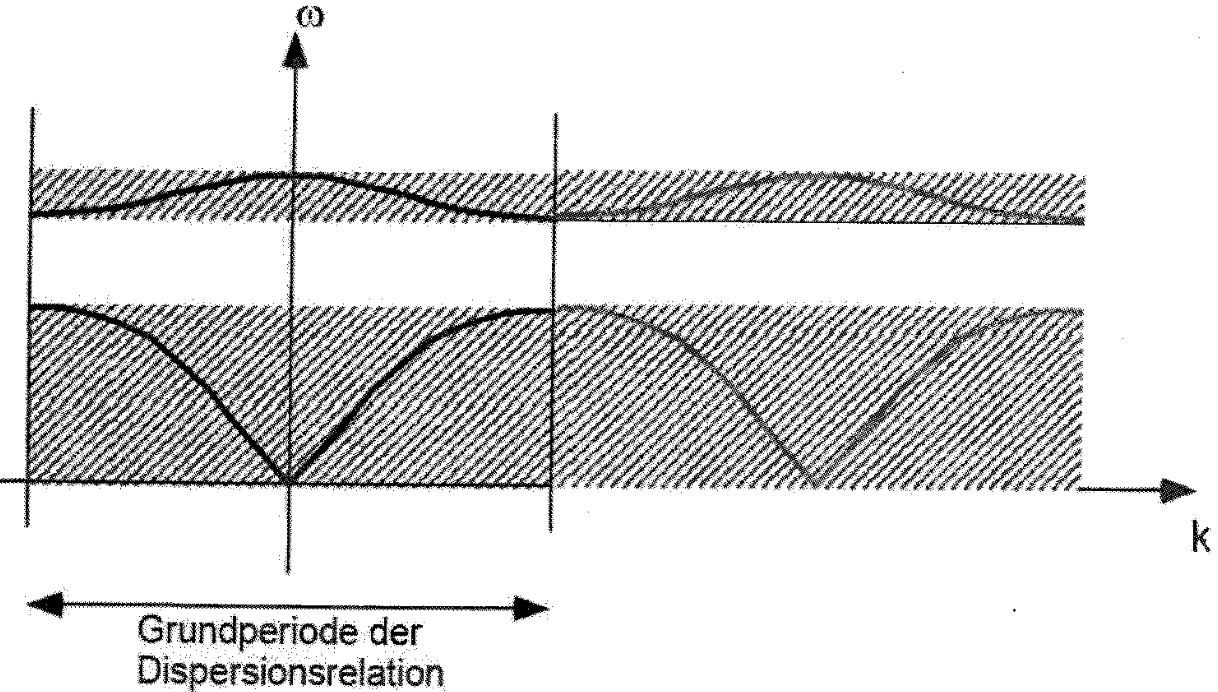
\includegraphics[width=0.6\textwidth]{fig/dispersionsrelation}
    \caption{Dispersionsrelation der diatomaren linearen Kette}
    \label{fig:dispersionsrelation}
\end{figure}

Anhand der Grafik lassen sich einige Punkte beobachten:
\begin{itemize}
    \item Es gibt Frequenzbereiche, in denen Wellen und Schiwnungen möglich sind (erlaubte Bänder)
    \item In den Frequenzlücken dazwischen ist keine Wellenausbreitung möglich (verbotete Zonen)
    \item Die Geschwindigkeit, mit der in diesem System Information transportiert werden kann, die
    sogenannte Gruppengeschwindigkeit, ist gegeben durch:
    \begin{equation}
        v_g=\frac{\partial \omega(k)}{\partial k}
    \end{equation}
    An den Bandrändern wird die Gruppengeschwindigkeit also $0$.
    \item Dispersionsrelationen können periodisch sein
\end{itemize}

\subsubsection{Effektive Masse (was ist schwerer, Elektron im Leitungsband oder Loch im Valenzband?)}
L\"ocher haben aufgrund des fehlenden Elektrons eine negative Masse, sind also eigentlich immer leichter als Elektronen.
Sollte die Frage Betragsmäßig gemeint sein, gibt es keine klare Antwort. Die effektive-Masse ist abhängig von der Kristallorientierung.

In der Praxis sind meist die Löcher schwerer (HAEgrula Saga, Seite 114).
\subsubsection{wo ist Elektron nach anheben ins Leitungsband bei indirektem HL (energetisch günstig!)}
Am minimum des Leitungsbandes.
\subsubsection{Gedankenexperiment: wenn Elektron in Leitungsband, und Valenzband voll besetzt, was passiert, wenn man HL abkühlt?}
Das Elektron muss oben bleiben, da unten ja kein Platz mehr ist.
\subsubsection{Zusammenhang zwischen Energie E und der Kreiswellenzahl k}
\begin{equation}
    E = \frac{(\hbar \cdot k)^2}{2m}
\end{equation}